\documentclass[12pt, oneside]{article}
\usepackage[letterpaper, margin=1in, headsep=0.5in, left=0.3in, right=2.5in]{geometry}
\usepackage[english]{babel}
\usepackage[utf8]{inputenc}
\usepackage{amsmath}
\usepackage{amsfonts}
\usepackage{amssymb}
\usepackage{tikz}
\usepackage{yhmath}
\usetikzlibrary{quotes, angles}
\usepackage{graphicx}
\usepackage{enumitem}
\usepackage{multicol}

\newif\ifmeta
\metatrue %print standards and topics tags

\title{Regents Geometry}
\author{Chris Huson}
\date{April 2022}

\usepackage{fancyhdr}
\pagestyle{fancy}
\fancyhf{}
\renewcommand{\headrulewidth}{0pt} % disable the underline of the header
\raggedbottom

%\fancyhead[LE]{\thepage}
\fancyhead[RO]{Name:}
\fancyhead[LO]{BECA / Dr. Huson / Geometry Regents Mixed Review}
\cfoot{\thepage}

\begin{document}
\subsubsection*{11.7 Similar triangles}
\begin{enumerate}[itemsep=2cm]
\item What are the coordinates of the center and the length of the radius of the circle whose equation is $(x+2)^2+(y-5)^2=81$? \vspace{1cm}
  
\item The equation of a cirle is $x^2+y^2-4x+10y=-20$. What are the center and radius of the circle?

\item In the diagram below of $\triangle ABC$ and $\triangle DEF$, angles $C$ and $F$ are right angles, and $\triangle ABC \sim \triangle DEF$
  \begin{center}
    \begin{tikzpicture}[scale=1]
    \draw [thick, xshift=4cm, yshift=2cm, rotate=208]
      (0,0)node[above]{$F$}--
      (4,0)node[below]{$E$}--
      (0,2.13)node[right]{$D$}--cycle;
      \draw [xshift=4cm, yshift=2cm, rotate=208]
        (0,0)++(0.3,0)--++(0,0.3)--+(-0.3,0);
    \draw [thick]
      (-1,-1)node[below]{$B$}--
      (-7,2)node[above]{$A$}--
      (-7,-1)node[below]{$C$}--cycle;
      \draw (-7,-1)++(0.3,0)--++(0,0.3)--+(-0.3,0);
  \end{tikzpicture}
  \end{center}
If $AC=10$, $BC=22$ and $DF=6$, what is the measure of $EF$?

\item In the diagram below of right triangle $KMI$, altitude $\overline{IG}$ is drawn to hypotenuse $\overline{KM}$.
  \begin{center}
    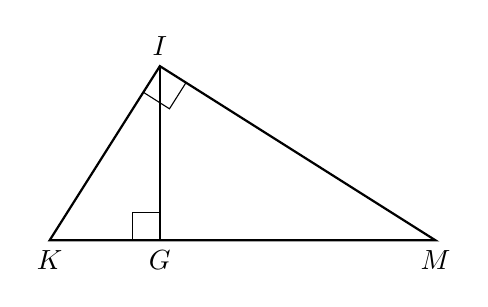
\begin{tikzpicture}[scale=0.7]
    \draw [thick]
    (0,0)node[below]{$K$}--
    (7,0)node[below]{$M$}--
    (2,3.16)node[above]{$I$}--cycle;
    \draw (2,3.16)++(-0.15*2,-0.15*3.16)--++(0.15*3.16,-0.15*2)--+(0.15*2,0.15*3.16);
    \draw [thick](2,0)node[below]{$G$}--(2,3.16);
    \draw (2,0)++(-0.5,0)--++(0,0.5)--+(0.5,0);
  \end{tikzpicture}
  \end{center}
IF $KG=4$ and $MG=9$, what is the length of $\overline{IG}$?

\newpage
\item Circle $O$ has chords $\overline{AD}$ and $\overline{BE}$ intersecting at $C$, as shown. Find $CD$.\\
  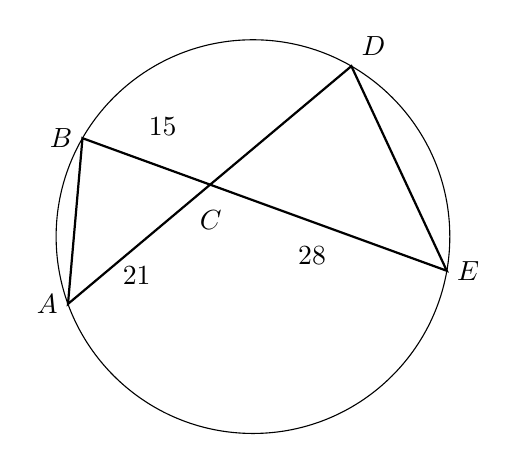
\begin{tikzpicture}[scale=0.5]
   \draw (0,0) circle[radius=5];
   \draw [thick]
   (-10:5) node[right] {$E$}--
   (150:5) node[left] {$B$}--
   (200:5) node[left] {$A$}--
   (60:5) node[above right] {$D$}--cycle;
   \draw (140:1.4) node[below] {$C$};
   \draw (125:4) node[below] {$15$};
   \draw (190:3) node[below] {$21$};
   \draw (0:1.5) node[below] {$28$};
  \end{tikzpicture}

\item Determine and state an equation of the line perpendicular to the line\\ $3x-5y=15$ and passing through the point $(1,5)$.
  
\item The endpoints of directed line segment $AB$ have coordinates of
$A(-5,-12)$ and $B(5,3)$. What are the coordinates of point $M$, on $\overline{AB}$, that divide $\overline{AB}$ into a ratio of 2:3?

\item At a distance of two miles, the angle of elevation to the top of a radio tower is $3.5^\circ$. \\[0.25cm]
What is the height of the tower, to the \emph{nearest foot}? (1 mile = 5280 feet)
  \begin{center}
    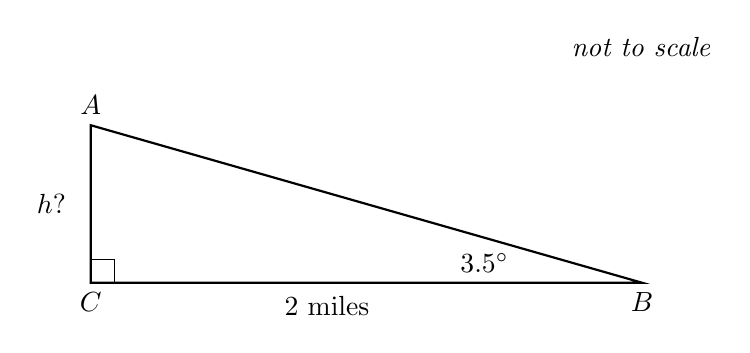
\begin{tikzpicture}[scale=1]
    \draw [thick]
      (0,0)node[below]{$B$}--
      (-7,2)node[above]{$A$}--
      (-7,0)node[below]{$C$}--cycle;
      \draw (-7,0)++(0.3,0)--++(0,0.3)--+(-0.3,0);
      \node at (-7.5,1){$h?$};
      \node at (-2,0.25){$3.5^\circ$};
      \node at (-4,-0.3){2 miles};
      \node at (0,3){\emph{not to scale}};
  \end{tikzpicture}
  \end{center}

\end{enumerate}
\end{document}
  